\newcommand{\package}{\emph}

\setcounter{chapter}{1}
\setcounter{section}{0}
\section{Evolutionary games}

\subsection{a}

Decide whether the pure strategies of a given payoff matrices are unbeatable etc

\textbf{Matrix i}

Strategy A is in:
\begin{itemize}
\item Strict Nash , because $5>3$ and $5>2$ 
\item It also means that it is in ESS, weak ESS and Nash
\item Not unbeatable because ($5>3$ and $3>1$) is true but ($5>2$ and $1>1$) is not true
\end{itemize}

Strategy B is in:
\begin{itemize}
\item Neither in any equilibrium because it does not satisfy the weakest condition of Nash equilibrium (i.e. neither of $1>3$, $1>2$ are true )
\end{itemize}

Strategy C is in:
\begin{itemize}
\item Nash equilibrium ( $1>0$ and $1\geq 1$)
\item Not in weak ESS because $1=1$ but not $2\geq 5$)
\item So, neither higher order equilibrium is applicable
\end{itemize}

\textbf{Matrix ii}

Strategy A is in:
\begin{itemize}
\item neither equilibrium, because $4>3$ but not $4>5$
\end{itemize}

Strategy B is in:
\begin{itemize}
\item neither any equilibrium, because  $1>0$ but not $1>2$ 
\end{itemize}

Strategy C is in:
\begin{itemize}
\item neither any equilibrium, because  $2>1$ but not $2>3$
\end{itemize}

\textbf{Matrix iii}

Strategy A is in:
\begin{itemize}
\item Neither in any equilibrium, because $-2 > 0$ is not true
\end{itemize}

Strategy B is in:
\begin{itemize}
 \item Neither in any equilibrium, because $2>4$ is not true
\end{itemize}

Strategy C is in:
\begin{itemize}
\item Nash equilibrium, because both are true: $2\geq 2$ and $2>-2$
\item Weak ESS, because it is true that  $2=2$ and $2=2$
\item Not in any other equilibriums
\end{itemize}

\textbf{Matrix iv}

Strategy A is in:
\begin{itemize}
\item Not in strict Nash because $2>2$ is not true (so not unbeatable as well)
\item In ESS because $2>1$ and ($2=2$ and $3>1$) so in weak ESS and Nash as well
\end{itemize}

Strategy B is in:
\begin{itemize}
\item Neither in any equilibrium, because  $1>3$ is not true
\end{itemize}

Strategy C is in:
\begin{itemize}
\item Neither in any equilibrium, because $1>3$ is not true
\end{itemize}

\subsection{b}

both A and B are not in Nash equilibrium because $0>2$ (not true) and $0>1$ (not true)
In case we allow playing a third mixed strategy $S=pA+(1-p)B$ we could rewrite the payoff matrix as follows:

\begin{tabular}{|c|c|c|c|}
\hline \rule[-2ex]{0pt}{5.5ex}  & A & B & S \\ 
\hline \rule[-2ex]{0pt}{5.5ex} A & 0 & 1 & $0p+(1-p)1$ \\ 
\hline \rule[-2ex]{0pt}{5.5ex} B & 2 & 0 & $2p+(1-p)0$ \\ 
\hline \rule[-2ex]{0pt}{5.5ex} S & $0p+(1-p)2$ & $1p+(1-p)0$ & $0p+(1-p)2*p+(2p+1p+((1-p)0)*(1-p)$ \\ 
\hline 
\end{tabular} 

Then after some algebraic transformation we have

\begin{tabular}{|c|c|c|c|}
\hline \rule[-2ex]{0pt}{5.5ex}  & A & B & S \\ 
\hline \rule[-2ex]{0pt}{5.5ex} A & 0 & 1 & $1-p$ \\ 
\hline \rule[-2ex]{0pt}{5.5ex} B & 2 & 0 & $2p$ \\ 
\hline \rule[-2ex]{0pt}{5.5ex} S & $2-2p$ & $p$ & $3p-3p^2$ \\ 
\hline 
\end{tabular} 


So, the necessary conditions for mixed strategy $S$ to be in Nash are 

$3p-3p^2 \geq 1-p$, after some transformations: $3p(1-p) \geq 1-p$, then $3p\geq 1$ , so $p \geq 1/3$

and

$3p-3p^2 \geq 2p$, after some transformations: $3-3p \geq 2$, then $1 \geq 3p$, so $p\leq \frac{1}{3}$.

So, we can see that the only $p$ which satisfy for inequalities is $p=\frac{1}{3}$.

Solution: mixed strategy is in Nash equilibrium with $p=\frac{1}{2}$ 



\setcounter{chapter}{2}
\setcounter{section}{0}
\section{Lotka-Volterra equation}

\subsection{a}
Solving the equations for x'=0 and y'=0

\begin{align*}
x'&=x(a-by)\\
y'&=y(-c+dx)
\end{align*}


yields in the following fixed points:
 
\begin{align*}
x &= 0, y =0 \\
x &= \frac{c}{d} , y = \frac{a}{b}
\end{align*}

The first points retrieved represent the condition when no species exists, while the second points refer to the situation where we observe the coexistance of both predator and prey. This situation depends on the values of parameters $a,b,c,d$.

\subsection{b}

To analyse the stability of the non-trivial points we have to write the jacobian matrix of the right-hand-side of the equation:
\[J = \begin{pmatrix}
\frac{\partial x}{\partial x} & \frac{\partial x}{\partial y}\\
\frac{\partial y}{\partial x} & \frac{\partial y}{\partial y}\\
\end{pmatrix}\]

Where 

\begin{align*}
\frac{\partial x}{\partial x}  &= \frac{\partial}{\partial x}(x(a-by)) = a-by\\
\frac{\partial x}{\partial y}  &= \frac{\partial}{\partial y}(x(a-by)) = -xb\\
\frac{\partial y}{\partial x}  &= \frac{\partial}{\partial x}(y(-c+dx)) = yd\\
\frac{\partial y}{\partial y}  &= \frac{\partial}{\partial y}(y(-c+dx)) = -c+dx
\end{align*}

\[J = \begin{pmatrix}
a-by & -xb\\
yd & -c+dx\\
\end{pmatrix}\]

When $x'= \frac{c}{d}$ and $y'=\frac{a}{b}$, then:

\[J^*= \begin{pmatrix}
0 & -\frac{bc}{d}\\
\frac{ad}{b} & 0\\
\end{pmatrix}\]

Hence, the eigenvalues:

\[ det(j^*-\lambda I) = (-\lambda)(-\lambda) - (-\frac{bc}{d})(\frac{ad}{b}) = \lambda^2 +ac \]
\[ \lambda = i\sqrt{ac} \text{ and } \lambda = -i\sqrt{ac} \]

The real part is the defined in $0$ while the immaginary part in $\pm i \sqrt{ac}$.

When eigenvalues are of the form $a + bi$, where $a$ and $b$are real scalars and $i$ is the imaginary number $\sqrt{-1}$, there are three important cases. These three cases are when the real part $a$ is positive, negative, and zero. In all cases, when the complex part of an eigenvalue is non-zero, the system will be oscillatory. When the real part is zero, the system behaves as an undamped oscillator. This can be visualized in two dimensions as a vector tracing a circle around a point. The plot of response with time would look sinusoidal. The figures below should help in understanding\footnote{\url{https://controls.engin.umich.edu/wiki/index.php/EigenvalueStability\#Imaginary_.28or_Complex.29_Eigenvalues}}.

Hence the point is not attractive and the population will oscillate in a close vicinity of the fixed point without approching it. 

\subsection{c}

Starting from a general Lotka Volterra Equation for $n$ species $y_i$ with real coefficients $r_i$, $b_{ij}$:

\[  y'_i  = y_i(r_{i}+\sum\limits_{j=1}^{n} b_{ij}y_j)  \]
\[ r_i = a_{in+1} - a_{n+1n+1} \text{~~~~~~} b_{ij} = a_{ij} - a_{n+1j} \]


Replicator equation for $n+1$ strategies $x_i$:

\[ x'_i = x_i(f_i(x) - \theta (x) \text{~~~~where~~~~} f_i(x) = \sum\limits_{j=1}^{n+1} x_ja_{ij} \theta(x) = \sum\limits_{j=1}^{n+1} x_if_i(x)\]

\[ \text{If~~~~} y = \sum\limits_{i=1}^{n} y_i \text{~~~and~~~} x_i = \frac{y_i}{1+\sum\limits_{j=1}^{n} y_j} = \frac{y_i}{1+y} \text{;} x_{n+1} = \frac{1}{1+\sum\limits_{j=1}^{n}y_j} = \frac{1}{1+y}\]

We have

\begin{align*}
(\frac{x_i}{x_{n+1}}) &= \frac{x_ix_{n+1}-x_{n+1}x_i}{(x_{n+1})^2} = \frac{x_i(fi(x)-\theta(x))x_{n+1} -x{x+1}(f_{n+1}(x)-\theta(x))x_i}{(x_{n+1})^2}\\
\left(\frac{\frac{y_i}{1+y}}{\frac{1}{1+y}}\right) &= \frac{x_ix_{n+1}(f_i(x)-\theta(x)-f_{n+1}(x)+\theta(x))}{(x_{n+1})^2}\\
y'_i &= \frac{x_i}{x_{n+1}}(f_i(x)-f_{n-1}(x)) = \frac{\frac{y_i}{1+y}}{\frac{1}{1+y}}\left(\sum\limits_{j=1}^{n+1}\frac{y_j}{1+y}a_{ij} - \sum\limits_{j=1}^{n+1}\frac{y_j}{1+y}a_{n+1j}\right)\\
y'_i &= y_i \left( \sum\limits_{j=1}^{n+1}\frac{y_j}{1+y}(a_{ij}-a_{n+1}) \right) = y_i\frac{1}{1+y} \left( \sum\limits_{j=1}^{n+1} {y_j}(a_{ij}-a_{n+1}) \right)
\end{align*}

Due to the fact that $\frac{1}{1+y}$ affects only the speed at which the trajectory is travelled, we can rewrite it in the following way:
\begin{align*} 
y'_i &= y_i \left( \sum\limits_{j=1}^{n+1} y_j(a_{ij}-a_{n+1j}) \right) = y_j \left( y_{n+1}(a_{in+1}-a_{n+1n+1}) + \sum\limits_{j=1}^{n} y_j(a_{ij}-a_{n+1j})\right)\\
y'_i &= y_i(1*r_i + \sum\limits_{j=1}^{n} b_{ij}y_{j}) = y_i\left(r_i+\sum\limits_{j=1}^{n} b_{ij}y_j \right)
\end{align*}

\setcounter{chapter}{4}
\setcounter{section}{0}
\section{Weak selection}
\begin{figure}[hp]
\centering
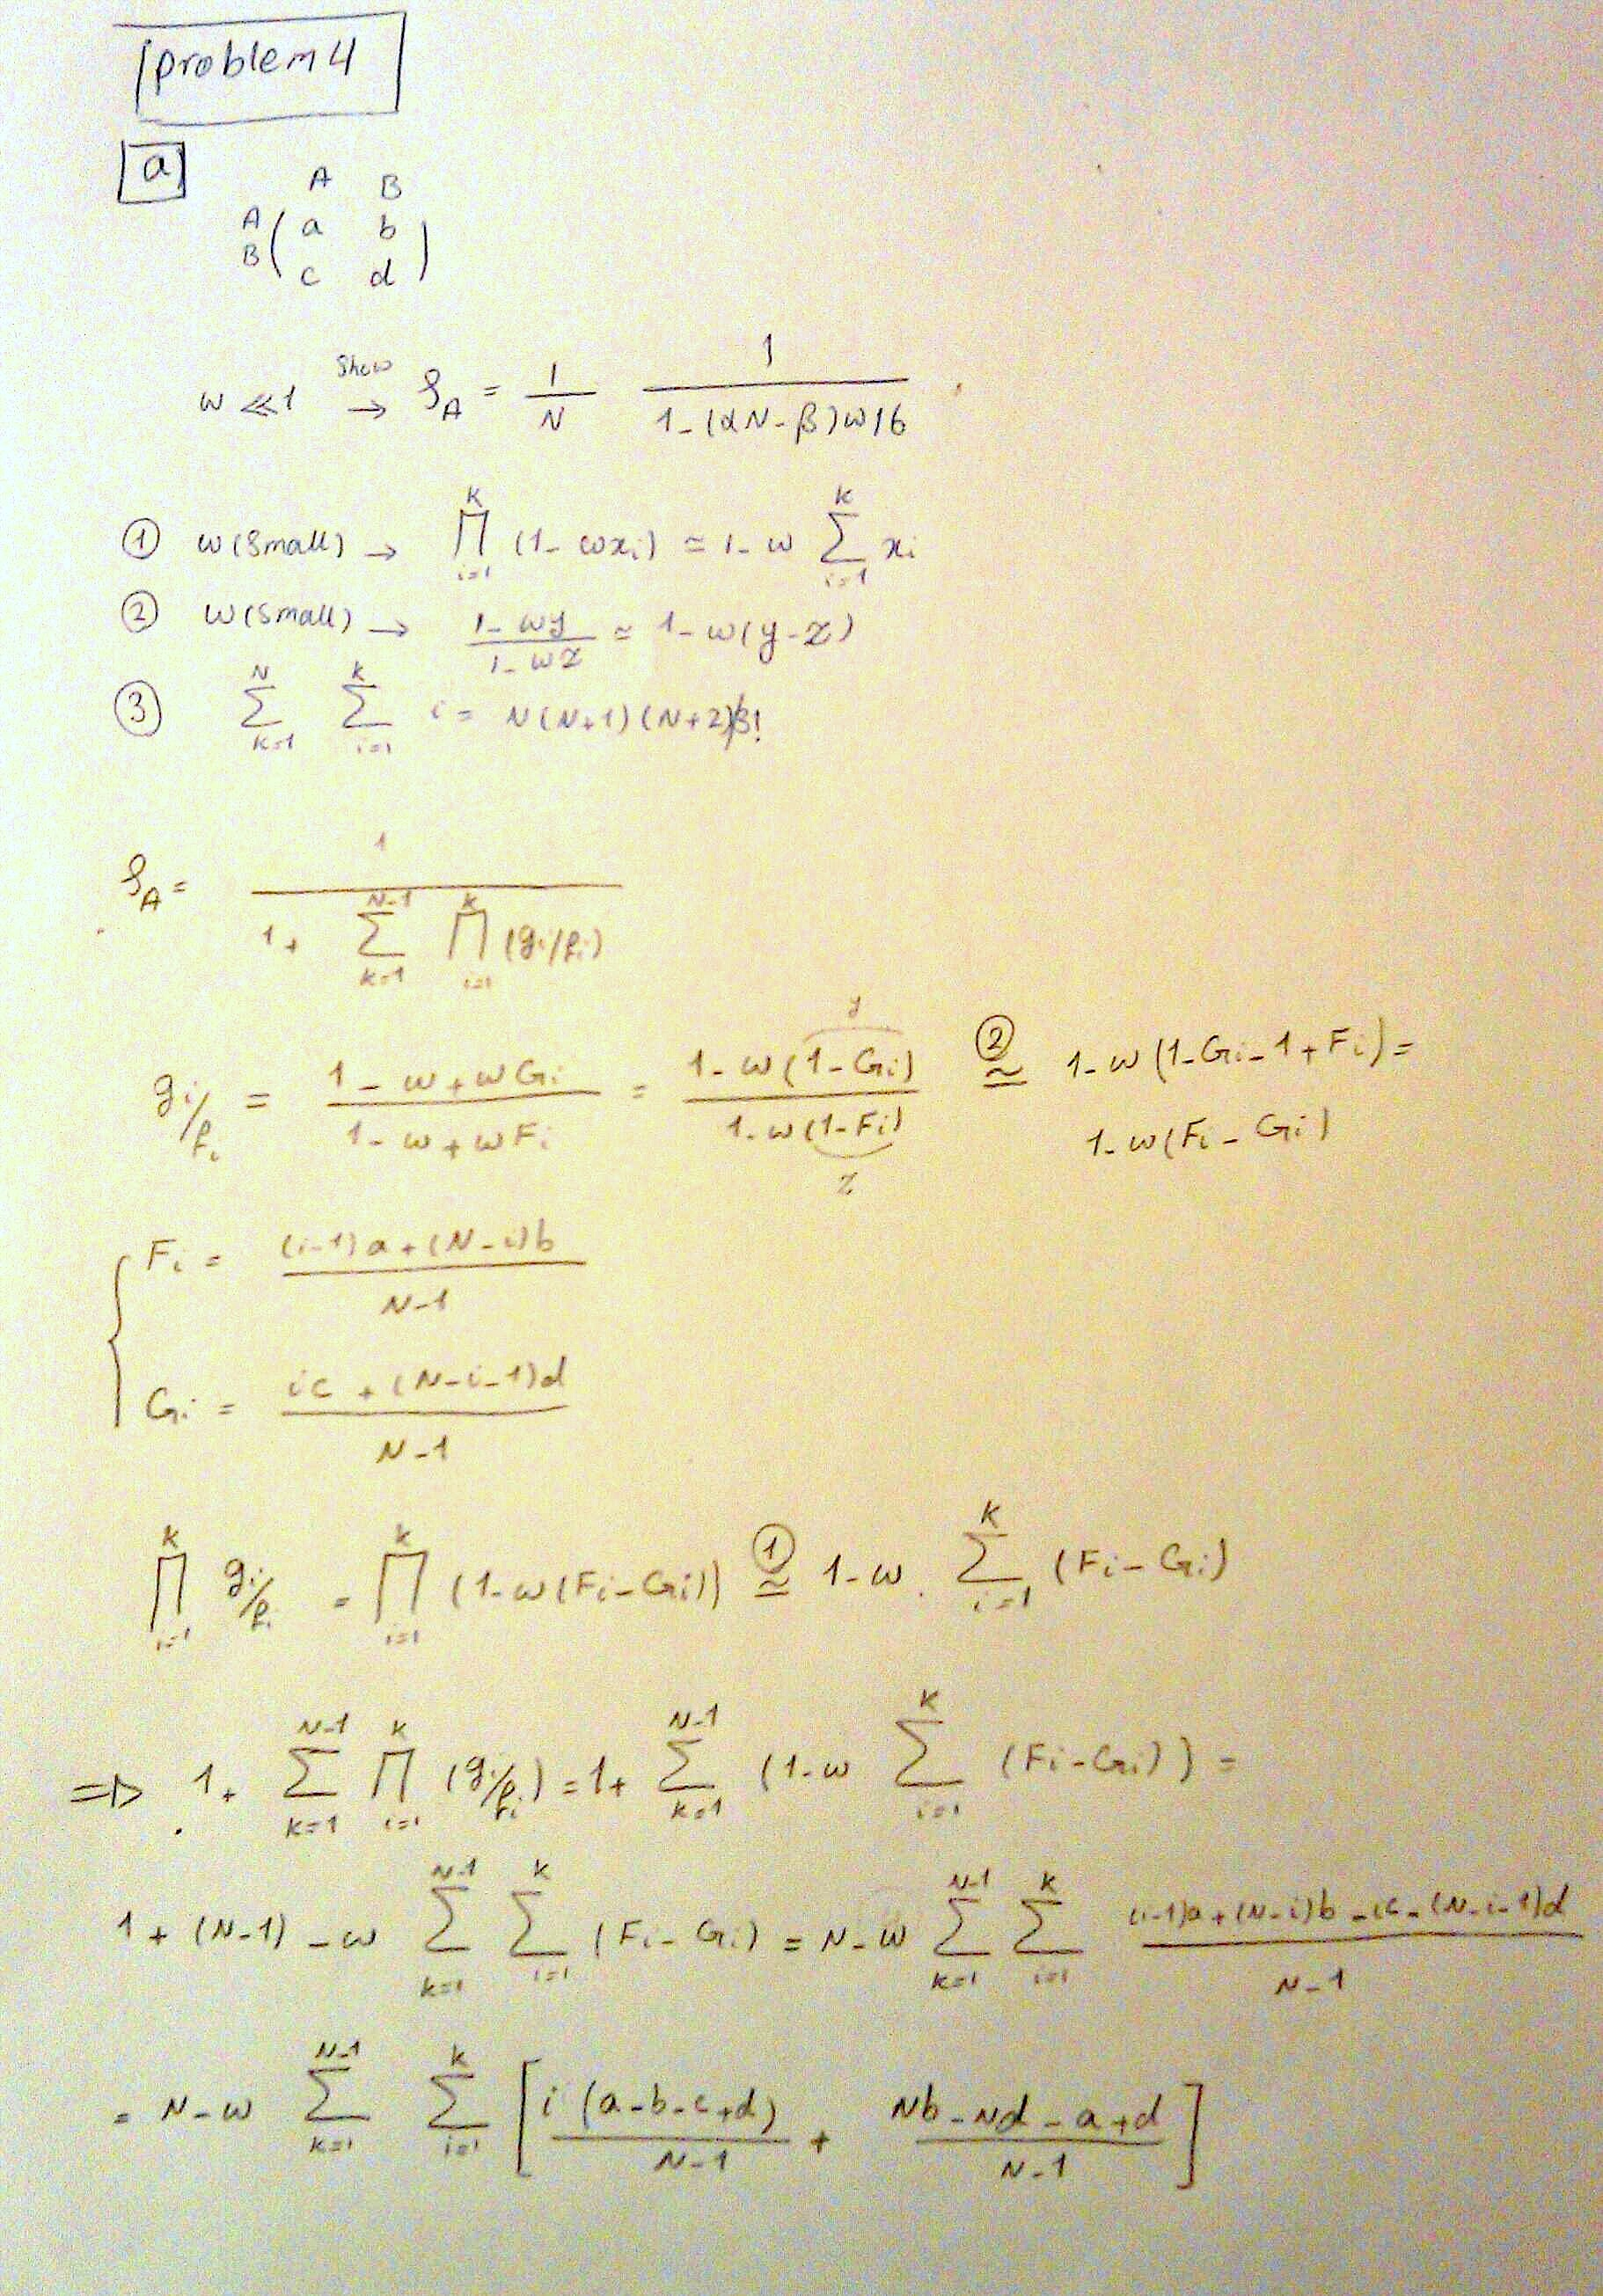
\includegraphics[scale=0.23]{./img/1}
\end{figure}
\begin{figure}[hp]
\centering
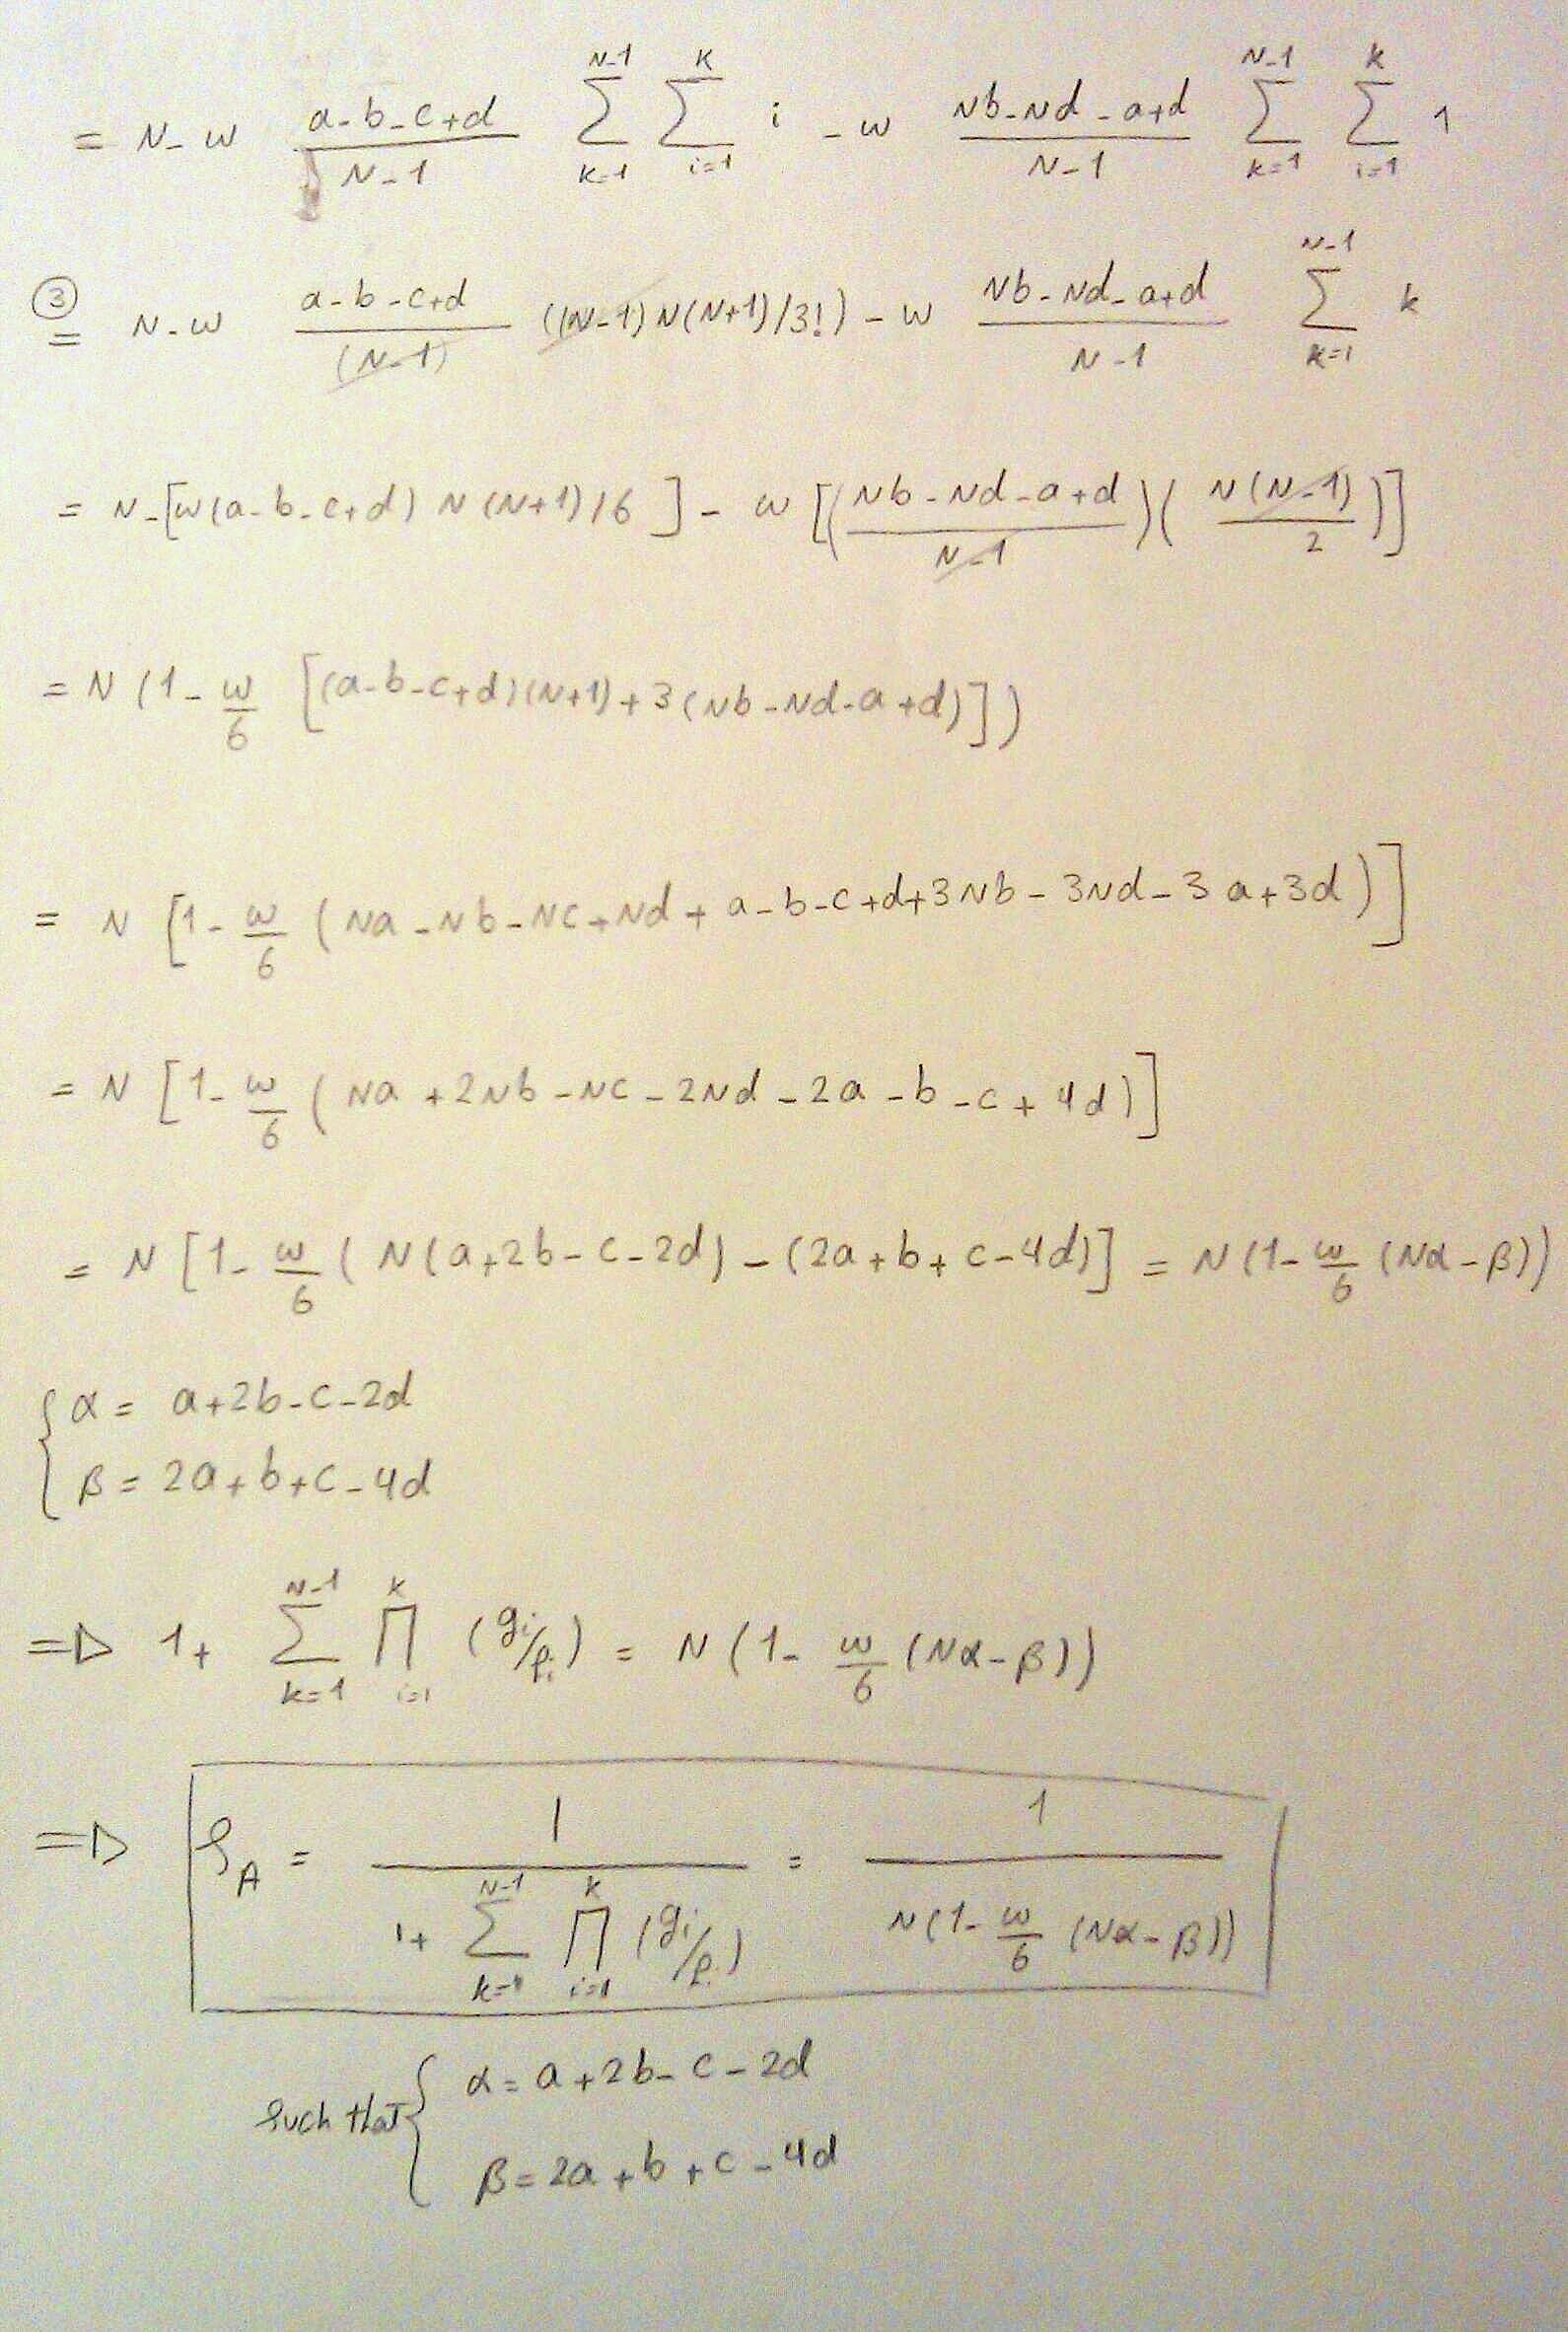
\includegraphics[scale=0.25]{./img/2}
\end{figure}
\begin{figure}[hp]
\centering
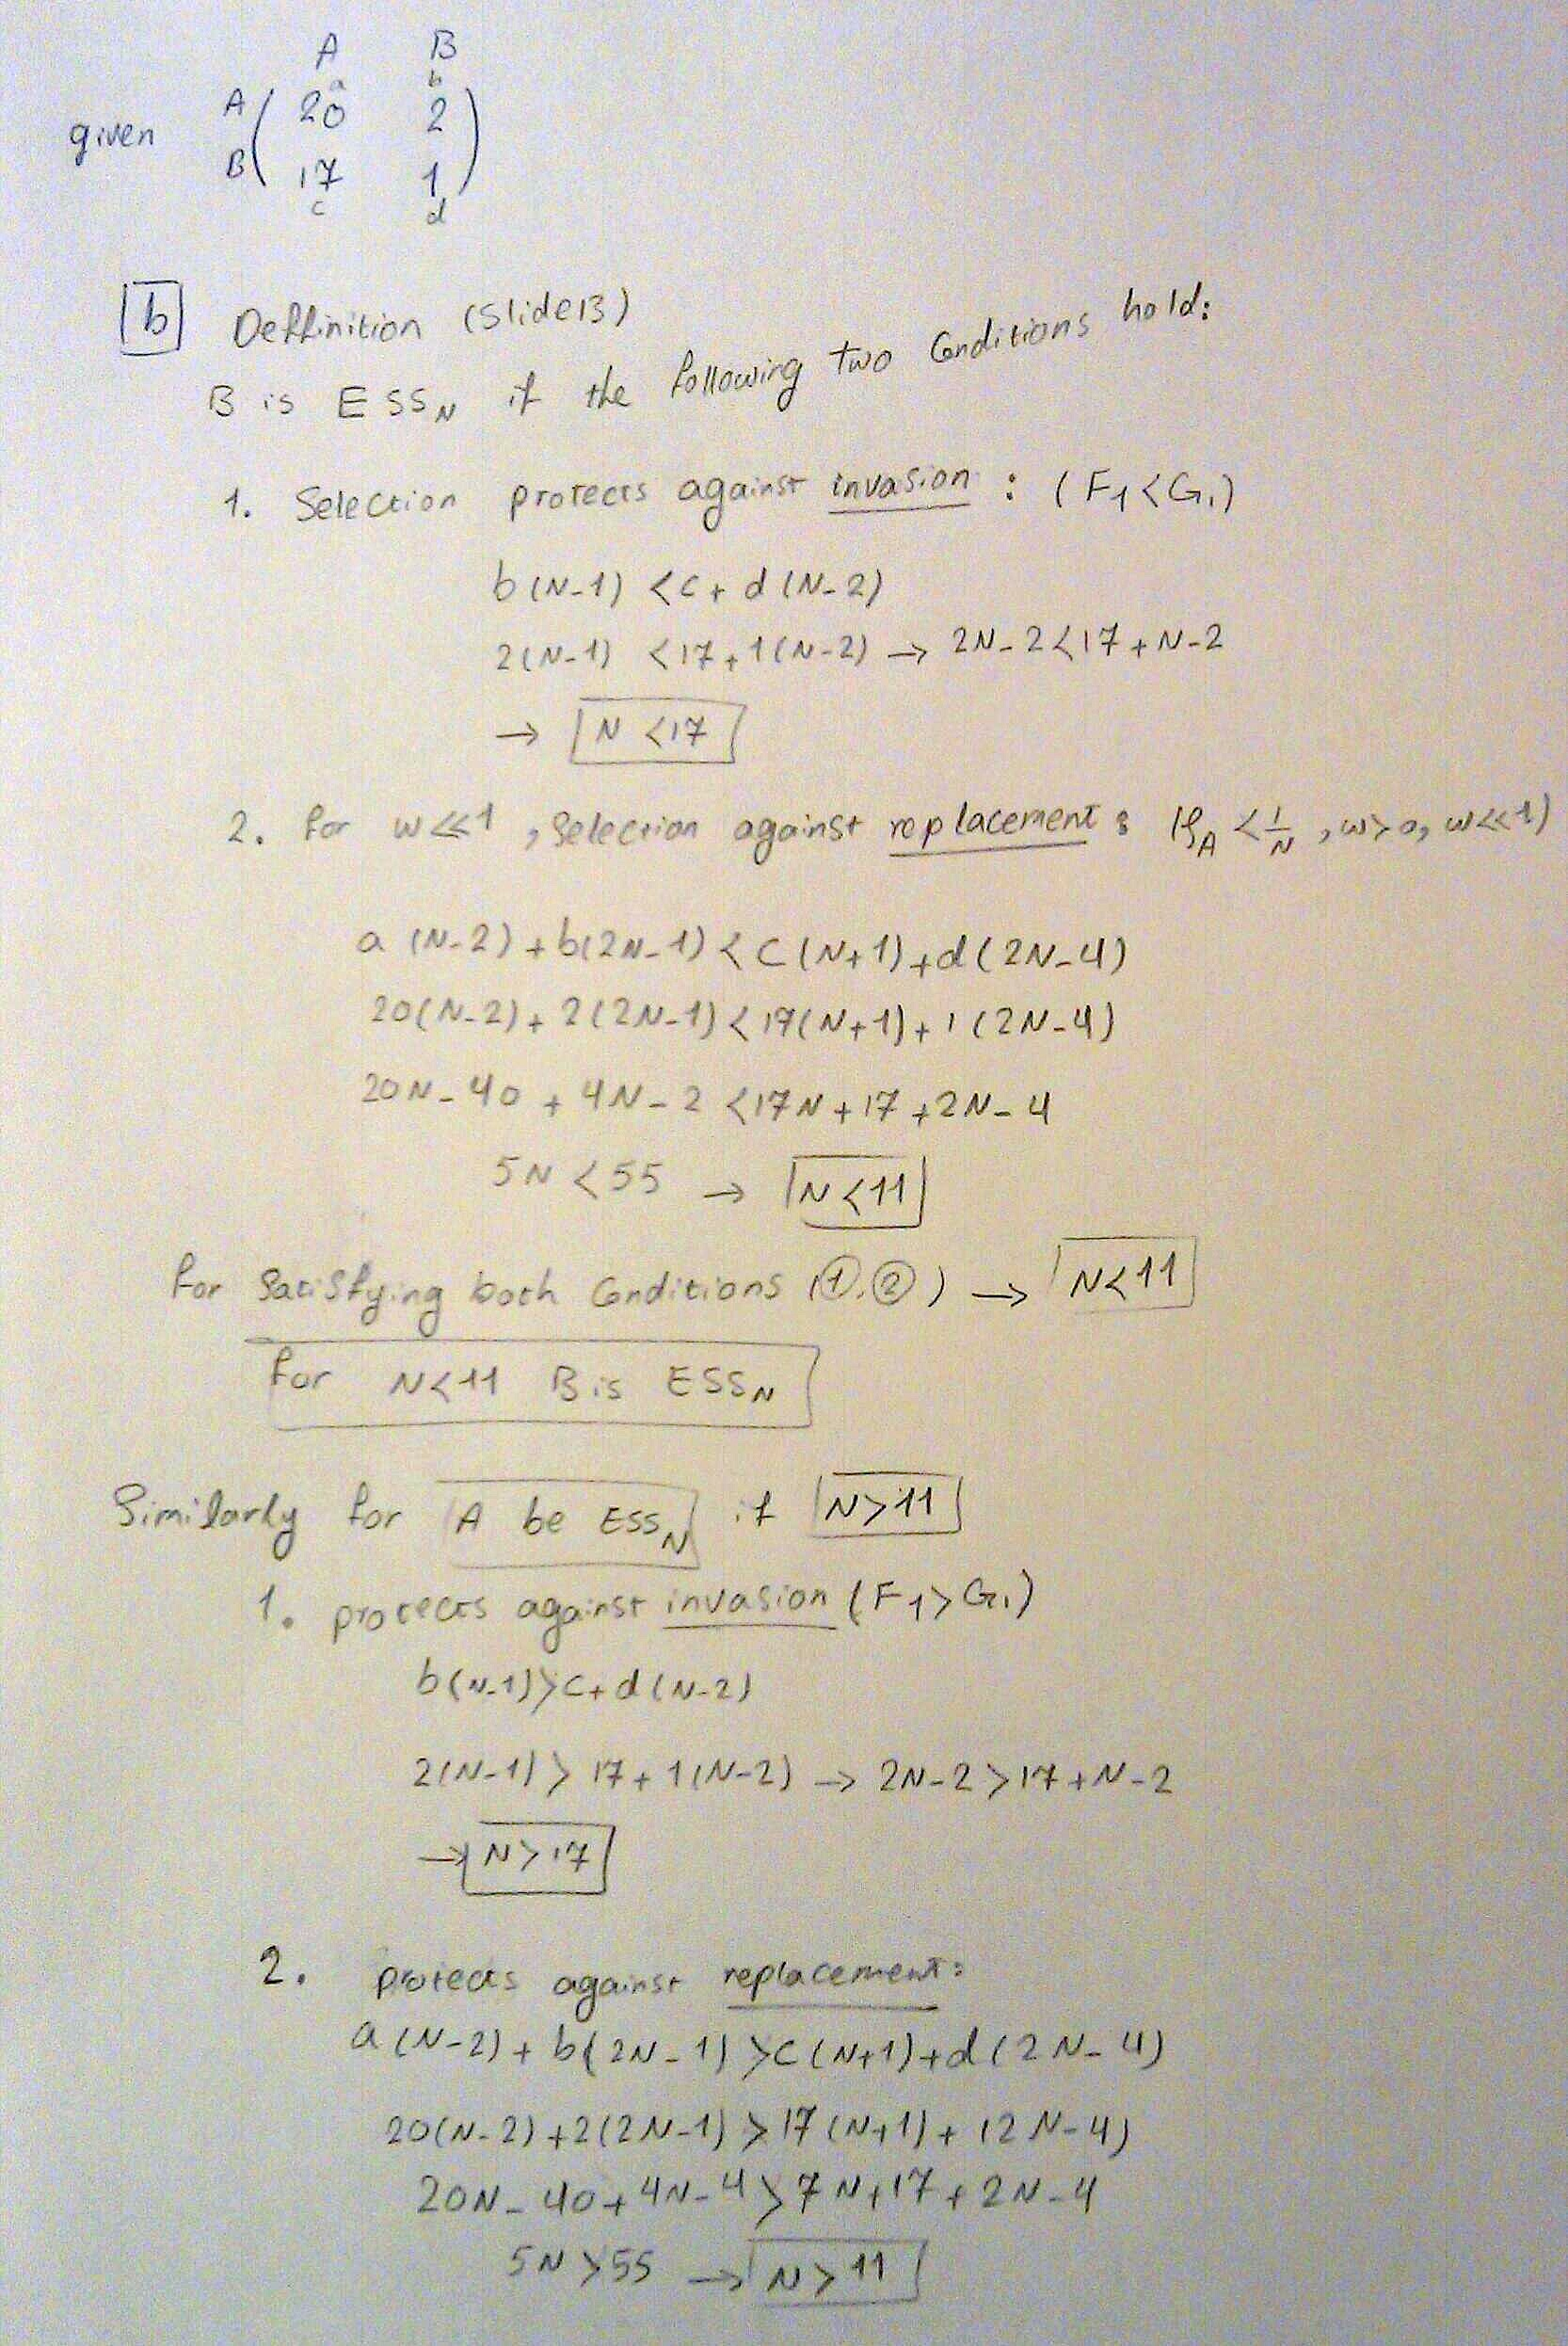
\includegraphics[scale=0.24]{./img/3}
\end{figure}
\begin{figure}[hp]
\centering
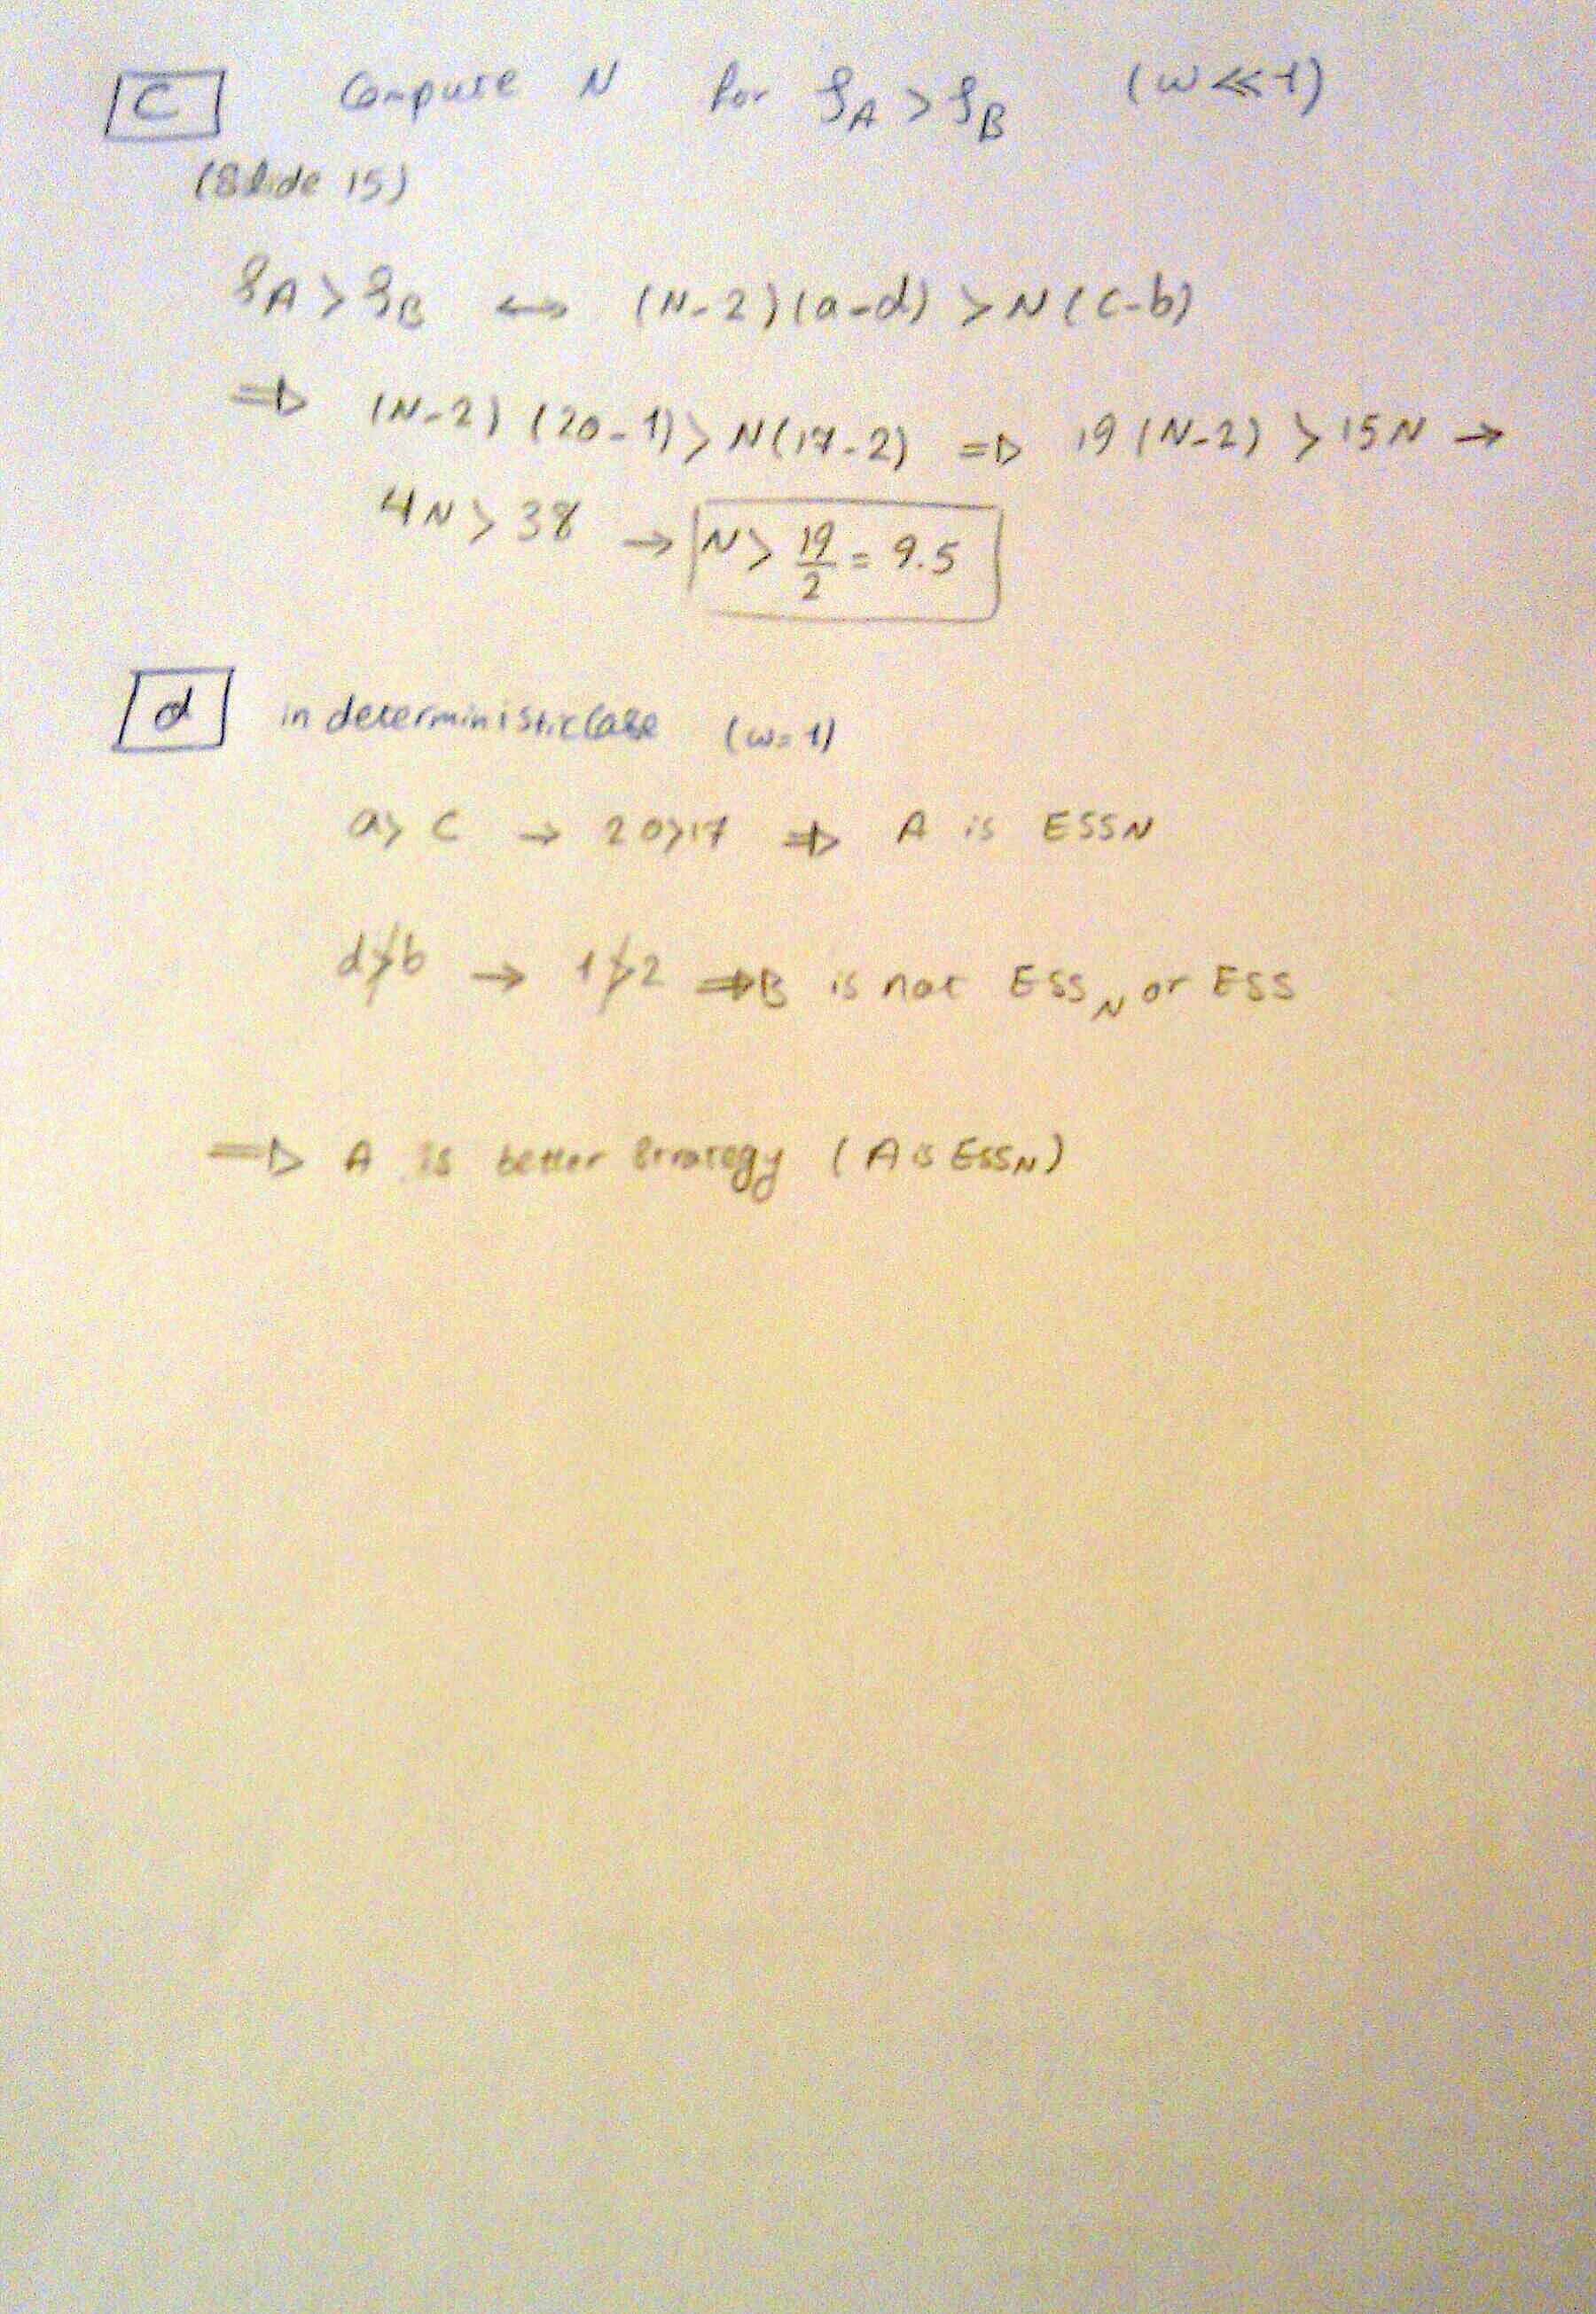
\includegraphics[scale=0.23]{./img/4}
\end{figure}
